\documentclass[12pt, a4paper]{article}
\usepackage[russian]{babel}
\usepackage{fontspec}
\setsansfont{Calibri}
\setmonofont{Consolas}
\setmainfont[
    Ligatures=TeX,
    Extension=.otf,
    BoldFont=cmunbx,
    ItalicFont=cmunti,
    BoldItalicFont=cmunbi,
]{cmunrm}
\usepackage{polyglossia}
\setdefaultlanguage{russian}
\setotherlanguage{english}


\usepackage{geometry}
\usepackage{pgfplotstable}

\geometry{
margin=2cm
}


\usepackage{indentfirst}

\usepackage{arydshln}
\usepackage[fleqn]{amsmath}
\usepackage{xfrac}
\usepackage{esint}
\usepackage{amssymb}
\usepackage{mathbbol}
\usepackage[T1]{fontenc}
\usepackage{mathtools}
\usepackage{color}
\usepackage{ulem}
\usepackage{tabu}
\usepackage{multicol}
\usepackage{multirow}
\usepackage{rotating}

\usepackage[outline]{contour}
\contourlength{1.2pt}

%\usepackage{tikz}
\usepackage{graphics}
\usepackage{xcolor}

\usepackage{pgfplots}
\usepackage{pgfplotstable}


\usepackage[at]{easylist}

\DeclareMathOperator{\sign}{sign}

%-------------------------------------------------------------------------------
%-------------------------------------------------------------------------------
%-------------------------------------------------------------------------------


\newcommand{\insertTitle}[7]{
\begin{titlepage}
	\begin{center}
    	\large
		Министерство науки и высшего образования Российской Федерации
		
		Новосибирский государственный технический университет
		%\vspace{0.25cm}
		\vfill
		{\textbf #1}
		
		Лабораторная работа №#2
		\vfill
	\end{center}
	
	\begin{tabular}{ m{7em}  m{7em} }
	Факультет: & ФПМИ \\ 
	Группа: & #3 \\  
	Студенты: & #4 \\
	& #5 \\
	Вариант: & #6
	\end{tabular}
	\vfill

\begin{center}
Новосибирск

#7
\end{center}
\end{titlepage}
}


\pgfplotstableset{
%\rowcolors{2}{gray!25}{white}
	begin table={\begin{tabular}},
	end table=\end{tabular},
}



\newcommand{\inputTableE}[1]{
\begin{center}
\noindent
\pgfplotstabletypeset[
	columns/E/.style={column name={$\varepsilon$},},
	columns/iter/.style={column name={\scriptsize Итераций},},
	columns/fCalc/.style={column name={\scriptsize Вычислений $f$},},
	columns/r/.style={column name={\scriptsize r},},
	columns/x/.style={string type, column name={$\mathbf{x}$},},
	columns/fx/.style={column name={$f(\mathbf{x})$}, column type/.add={}{|},},
	every head row/.style={before row=\hline,after row=\hline\hline}, 
	every last row/.style={after row=\hline},
	column type/.add={|}{},
	col sep=tab,
]{#1}
\end{center}
}


\newcommand{\inputTableRFirst}[1]{
\begin{center}
\noindent
\pgfplotstabletypeset[
	columns/rFirst/.style={column name={$r_0$},},
	columns/iter/.style={column name={\scriptsize Итераций},},
	columns/fCalc/.style={column name={\scriptsize Вычислений f},},
	columns/r/.style={column name={\scriptsize r},},
	columns/x/.style={string type, column name={$\mathbf{x}$},},
	columns/fx/.style={column name={$f(\mathbf{x})$}, column type/.add={}{|},},
	every head row/.style={before row=\hline,after row=\hline\hline}, 
	every last row/.style={after row=\hline},
	column type/.add={|}{},
	col sep=tab,
]{#1}
\end{center}
}


\newcommand{\inputTableRMult}[1]{
\begin{center}
\noindent
\pgfplotstabletypeset[
	columns/rMult/.style={column name={$rMult$},},
	columns/iter/.style={column name={\scriptsize Итераций},},
	columns/fCalc/.style={column name={\scriptsize Вычислений $f$},},
	columns/r/.style={column name={\scriptsize r},},
	columns/x/.style={string type, column name={$\mathbf{x}$},},
	columns/fx/.style={column name={$f(\mathbf{x})$}, column type/.add={}{|},},
	every head row/.style={before row=\hline,after row=\hline\hline}, 
	every last row/.style={after row=\hline},
	column type/.add={|}{},
	col sep=tab,
]{#1}
\end{center}
}

\usepackage[utf8]{inputenc}
\usepackage{listings}
\usepackage{color}
 
\definecolor{codegreen}{rgb}{0,0.6,0}
\definecolor{codegray}{rgb}{0.5,0.5,0.5}
\definecolor{codepurple}{rgb}{0.58,0,0.82}
\definecolor{backcolour}{rgb}{0.85,0.85,0.85}
 
\lstdefinestyle{mystyle}{
	backgroundcolor=\color{backcolour},   
	commentstyle=\color{codegreen},
	keywordstyle=\color{blue},
	basicstyle=\fontsize{10}{12}\selectfont\ttfamily,
   	numberstyle=\tiny\color{codegray},
	stringstyle=\color{codepurple},
    	breakatwhitespace=false,         
	breaklines=true,                 
	captionpos=b,                    
	keepspaces=true,                 
	numbers=left,                    
	numbersep=5pt,                  
	showspaces=false,                
	showstringspaces=false,
	showtabs=false,                  
	tabsize=4
}
\lstset{ style=mystyle}


\newcommand{\funcGOne}[0]{
\[ G_j[g_j({\bar x})] = {\frac {1}{2}} {\bigl\{ {g_j({\bar x}) + {\bigl| g_j({\bar x}) }\bigr| \bigr\} }} \] }

\newcommand{\funcGTwo}[0]{
\[ G_j[g_j({\bar x})] = {\Bigl[ {\frac {1}{2}} {\bigl\{ {g_j({\bar x}) + {\bigl| g_j({\bar x}) }\bigr| \bigr\} }} \Bigr]}^2 \] }

\newcommand{\funcGThree}[0]{
\[ G_j[g_j({\bar x})] = {\Bigl[ {\frac {1}{2}} {\bigl\{ {g_j({\bar x}) + {\bigl| g_j({\bar x}) }\bigr| \bigr\} }} \Bigr]}^\alpha \text{,если } \alpha \text{ чётное}  \] }

\newcommand{\funcGFour}[0]{
\[ G_j[g_j({\bar x})] = {-\frac {1}{ g_j({\bar x}) } } \] }

\newcommand{\funcGFive}[0]{
\[ G_j[g_j({\bar x})] = {-ln \Bigl[{-g_j({\bar x})} \Bigr] } \] }



\newcommand{\funcInTextGOne}[0]{
$ G_j[g_j({\bar x})] = {\frac {1}{2}} {\bigl\{ {g_j({\bar x}) + {\bigl| g_j({\bar x}) }\bigr| \bigr\} }} $ }

\newcommand{\funcInTextGTwo}[0]{
$ G_j[g_j({\bar x})] = {\Bigl[ {\frac {1}{2}} {\bigl\{ {g_j({\bar x}) + {\bigl| g_j({\bar x}) }\bigr| \bigr\} }} \Bigr]}^2 $ }

\newcommand{\funcInTextGThree}[0]{
$ G_j[g_j({\bar x})] = {\Bigl[ {\frac {1}{2}} {\bigl\{ {g_j({\bar x}) + {\bigl| g_j({\bar x}) }\bigr| \bigr\} }} \Bigr]}^\alpha \text{,если } \alpha \text{ чётное}  $ }

\newcommand{\funcInTextGFour}[0]{
$ G_j[g_j({\bar x})] = {-\frac {1}{ g_j({\bar x}) } } $ }

\newcommand{\funcInTextGFive}[0]{
$ G_j[g_j({\bar x})] = {-ln \Bigl[{-g_j({\bar x})} \Bigr] } $ }



\newcommand{\myCodeInput}[3]{
{\bf #2}
\lstinputlisting[language=#1]{#3}
}

% Размер изображений [0, 1]
\newcommand{\picSize}{0.7}

\setlength{\abovedisplayskip}{-1pt}
\setlength{\belowdisplayskip}{-1pt}



\newcommand{\inputTwoImages}[2]{
\begin{figure}[htbp!]
    \noindent
        \includegraphics[width=0.48\textwidth]{#1}
        \includegraphics[width=0.48\textwidth]{#2}
\end{figure}

}


%-------------------------------------------------------------------------------
%-------------------------------------------------------------------------------
%-------------------------------------------------------------------------------


\begin{document}

%-------------------------------------------------------------------------------%-------------------------------------------------------------------------------
%-------------------------------------------------------------------------------
\insertTitle{Методы оптимизации}{3}{ПМ-63}{Кожекин М.В.}{Утюганов Д.С.}{5}{2019}




%-------------------------------------------------------------------------------%-------------------------------------------------------------------------------
%-------------------------------------------------------------------------------
\section{Цель работы}

Ознакомиться с методами штрафных функций при решении задач нелинейного программирования. Изучить типы штрафных и барьерных функций, их особенности, способы и области применения, влияние штрафных функций на сходимость алгоритмов, зависимость точности решения задачи нелинейного программирования от величины коэффициента штрафа.




%-------------------------------------------------------------------------------%-------------------------------------------------------------------------------
%-------------------------------------------------------------------------------
\section{Задание}

Применяя методы поиска минимума 0-го порядка, реализовать программу для решения задачи нелинейного программирования с использованием {\bf метода штрафных функций}. 

Исследовать сходимость {\bf метода штрафных функций} в зависимости от
\begin{itemize}
	\item[$-$] выбора штрафных функций,
	\item[$-$] начальной величины коэффициента штрафа,
	\item[$-$] стратегии изменения коэффициента штрафа,
	\item[$-$] начальной точки,
	\item[$-$] задаваемой точности.
\end{itemize}

Сформулировать выводы.

Применяя методы поиска минимума 0-го порядка, реализовать программу для решения задачи нелинейного программирования с ограничением типа неравенства {\bf (только пункт а)} с использованием {\bf метода барьерных функций}.

Исследовать сходимость {\bf метода барьерных функций (только пункт а)} в зависимости от

\begin{itemize}
	\item[$-$]выбора барьерных функций,
	\item[$-$]начальной величины коэффициента штрафа,
	\item[$-$]стратегии изменения коэффициента штрафа,
	\item[$-$]начального приближения,
	\item[$-$]задаваемой точности.
\end{itemize}

Сформулировать выводы.

{\bf Вариант 5}

При ограничении:

а) x + y <= -1

б) y = x + 1




%-------------------------------------------------------------------------------%-------------------------------------------------------------------------------
%-------------------------------------------------------------------------------
\section{Зависимость скорости сходимости метода от заданной точности}
%-------------------------------------------------------------------------------
\subsection{Штрафные функции}
\funcGOne{}
\inputTableE{tableE1.txt}
\funcGTwo{}
\inputTableE{tableE2.txt}
\funcGThree{}
\inputTableE{tableE3.txt}
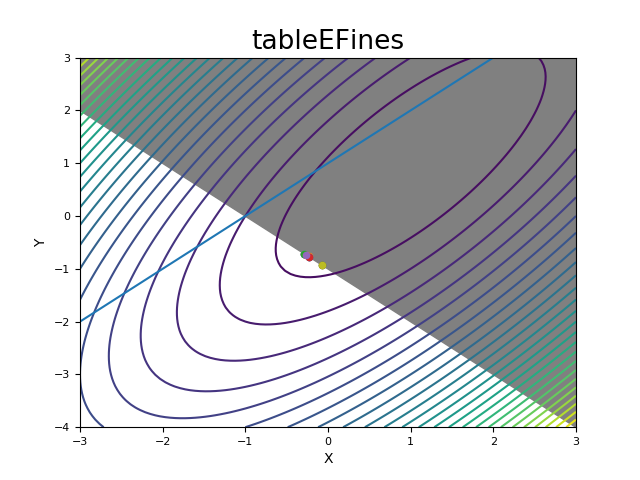
\includegraphics[width=\picSize\linewidth]{../pics/tableEFines.png}
%-------------------------------------------------------------------------------
\subsection{Барьерные функции}
\funcGFour{}
\inputTableE{tableE4.txt}
\funcGFive{}
\inputTableE{tableE5.txt}
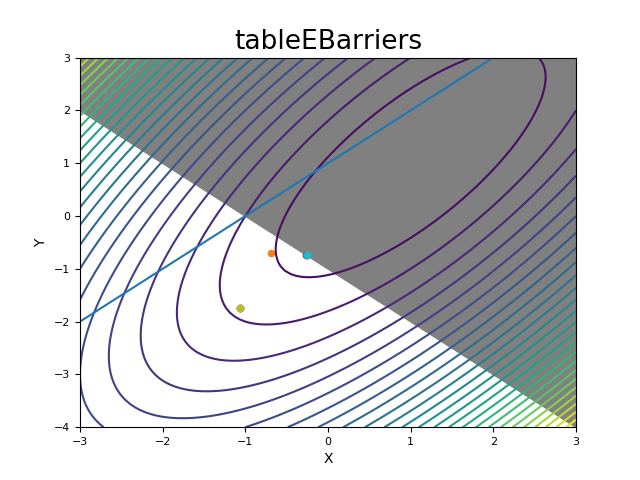
\includegraphics[width=\picSize\linewidth]{../pics/tableEBarriers.png}
%-------------------------------------------------------------------------------
\subsection{Вывод}

При значении малом значении $\alpha $ (0 и 1) заданная точность не оказывает влияние на скорость сходимости метода штрафных функций.

Для метода  барьерных функций рост точности ведёт к увеличению числа итераций и вычислений целевой функции.




%-------------------------------------------------------------------------------%-------------------------------------------------------------------------------
%-------------------------------------------------------------------------------
\section{Зависимость скорости сходимости метода от  коэффициента изменения штрафа}
%-------------------------------------------------------------------------------
\subsection{Штрафные функции}
\funcGOne{}
\inputTableRMult{tableRMult1.txt}
\funcGTwo{}
\inputTableRMult{tableRMult2.txt}
\funcGThree{}
\inputTableRMult{tableRMult3.txt}
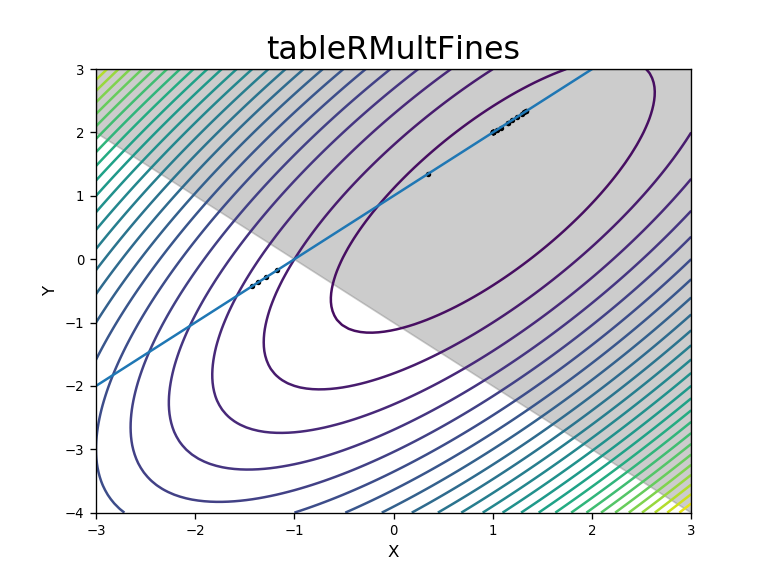
\includegraphics[width=\picSize\linewidth]{../pics/tableRMultFines.png}
%-------------------------------------------------------------------------------
\subsection{Барьерные функции}
\funcGFour{}
\inputTableRMult{tableRMult4.txt}
\funcGFive{}
\inputTableRMult{tableRMult5.txt}
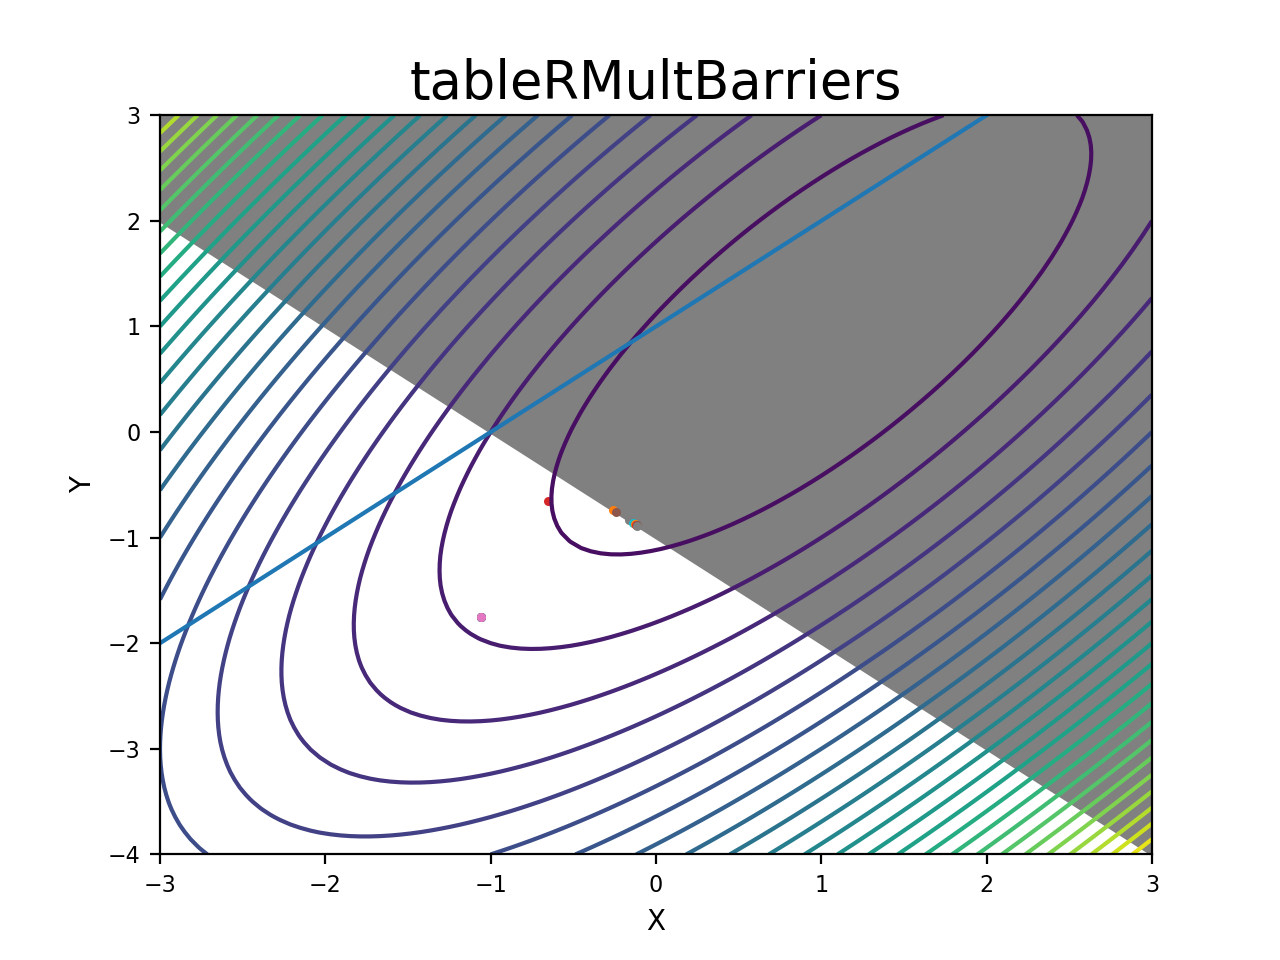
\includegraphics[width=\picSize\linewidth]{../pics/tableRMultBarriers.png}
%-------------------------------------------------------------------------------
\subsection{Вывод}
Рост коэффициента изменения штрафа ведёт к уменьшению числа итераций и вычислений целевой функции.

Оптимальным значением коэффициента штрафа является 4.




%-------------------------------------------------------------------------------
%-------------------------------------------------------------------------------
%-------------------------------------------------------------------------------
\section{Зависимость скорости сходимости метода от начального значения штрафа}
%-------------------------------------------------------------------------------
\subsection{Штрафные функции}
\funcGOne{}
\inputTableRFirst{tableRFirst1.txt}
\funcGTwo{}
\inputTableRFirst{tableRFirst2.txt}
\funcGThree{}
\inputTableRFirst{tableRFirst3.txt}
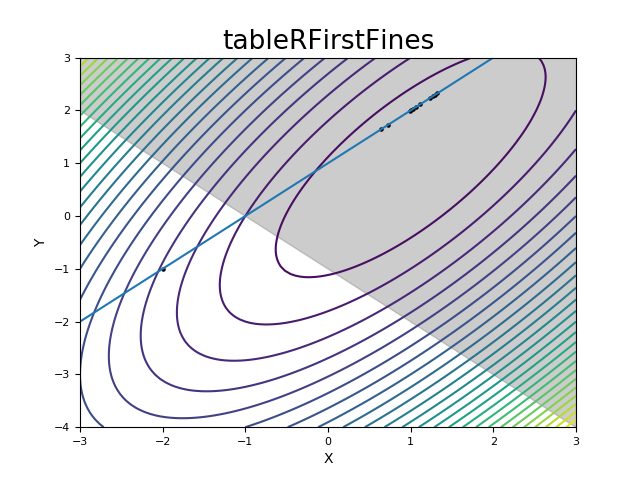
\includegraphics[width=\picSize\linewidth]{../pics/tableRFirstFines.png}
%-------------------------------------------------------------------------------
\subsection{Барьерные функции}
\funcGFour{}
\inputTableRFirst{tableRFirst4.txt}
\funcGFive{}
\inputTableRFirst{tableRFirst5.txt}
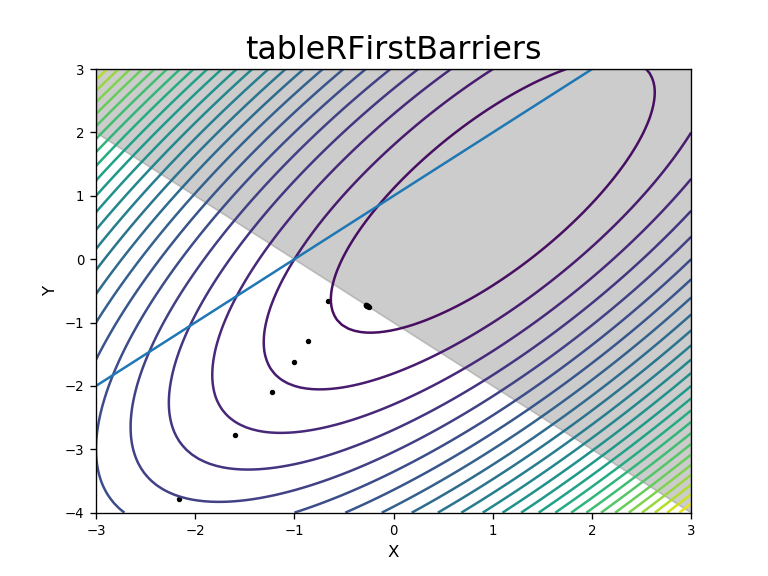
\includegraphics[width=\picSize\linewidth]{../pics/tableRFirstBarriers.png}
%-------------------------------------------------------------------------------
\subsection{Вывод}

Для решения методом штрафной функции оптимальным методом является выбор первой функции с начальным значением штрафа равным 4.

Для решения методом барьерной функции оптимален выбор штрафной функции с параметром

Для метода барьеров рост начального значения штрафа ведёт к тому, что метод в первую очередь стремится не найти локальный минимум, а стремится отойти как можно дальше от штрафной области.




%-------------------------------------------------------------------------------
%-------------------------------------------------------------------------------
%-------------------------------------------------------------------------------
\section{Зависимость скорости сходимости метода от начального приближения}

Параметры методов:
\begin{trivlist}
	\item $ E = 1e^{-12} $
	\item $ r_0 = 10 $
	\item $ rMult = 2 $
	\item $ \alpha = 8 $
\end{trivlist}

\inputTwoImages{../pics/Rosenbrock_Q1_1.png}{../pics/Rosenbrock_Q1_2.png}
\inputTwoImages{../pics/Rosenbrock_Q2_1.png}{../pics/Rosenbrock_Q2_2.png}
\inputTwoImages{../pics/Rosenbrock_Q3_1.png}{../pics/Rosenbrock_Q3_2.png}
\inputTwoImages{../pics/Rosenbrock_Q4_1.png}{../pics/Rosenbrock_Q4_2.png}
\inputTwoImages{../pics/Rosenbrock_Q5_1.png}{../pics/Rosenbrock_Q5_2.png}
%-------------------------------------------------------------------------------
\subsection{Вывод}

Начальное приближение слабо влияет на сходимость метода.



%-------------------------------------------------------------------------------
%-------------------------------------------------------------------------------
%-------------------------------------------------------------------------------
\section{Исходный код программы}
\myCodeInput{c++}{head.h}{../head.h}
\myCodeInput{c++}{main.cpp}{../main.cpp}
\myCodeInput{python}{plot.py}{../plot.py}

\end{document}